\documentclass{article}

\usepackage[T1]{fontenc}
\usepackage{graphicx}
\usepackage{fancyhdr}
\pagestyle{fancy}
\fancyhf{}
\lhead{Version 1.0}
\rhead{Elliot Oram}
\rfoot{\thepage}


\title{Charades Class Diagram}
\author{elo9@aber.ac.uk}

\begin{document}

\maketitle
\tableofcontents

\newpage

\section{Charades Class Diagram}
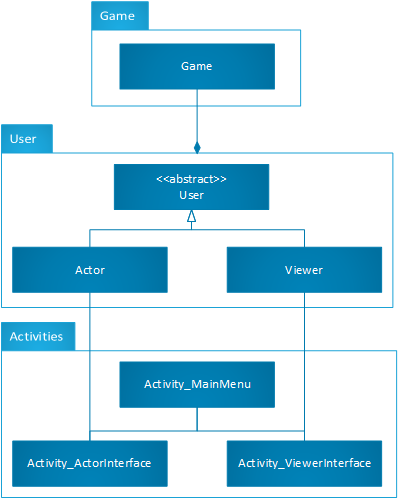
\includegraphics[width=\textwidth]{CharadesClassImage}

\newpage


\section{Description of Class Diagram}
\subsection{Game}
The Game package is currently a single class implementation. This will expand when more features are designed and built for the core game functionality. In essence, this class is designed to control the flow of information in the system. The class will deal with storing the current game state, as well as sending and receiving messages between the Viewers and Actors.


\subsection{User}
The User package models the possible users of the system. There is a User abstract class containing commonalities between all users and two concrete classes that inherit from this. The concrete classes represent the known users in the system the Actor, and the Viewer. 

Actor: The Actor will have the ability to pick a phrase or word and they will only see the actor specific interface.

Viewer: The Viewer will have the ability to guess the currently selected word or phrase and they will only see an instance of the viewer specific interface.

\subsection{Activities}
Activities are the andriod equivalent of graphical users interfaces. Each activity corresponds to a different screen on the app.

Activity MainMenu: The main menu activity will show the splash screen for the Charades Game.

Activity ActorInterface: The Actor interface will only be shown to the Actor in the the Staging Area, and will allow them to choose the phrase and current word to act out. The Actor will also be informed if the word or phrase they are acting has been guessed correctly. If the word they are acting has been guessed correctly, they will be asked to choose a new word from the remaining un-guessed words in the phrase.

Activity ViewerInterface: The Viewer interface will display the current word in the phrase that the viewer is attempting to guess, as well as the genre of the phrase (e.g. book, film, television show, ect.). This interface will give the option to guess either the word or the whole phrase and the page will contain a submit button to submit a guess. The interface will inform the viewer if the guess is correct or not. The interface will instruct the viewer to change places with the actor if they guess the phrase correctly.

\end{document}